\documentclass[12pt]{article}
\usepackage{amssymb,amsmath,cite,geometry,graphicx,url}
\addtolength{\textheight}{.8in}
\addtolength{\textwidth}{.9in}
\addtolength{\topmargin}{-.4in}
\addtolength{\evensidemargin}{-.45in}
\addtolength{\oddsidemargin}{-.45in}

\catcode`\@=11

%       This causes equations to be numbered by section

\@addtoreset{equation}{section}
\def\theequation{\arabic{section}.\arabic{equation}}

%       reset section commands

\catcode`\@=11
\def\thesection{\arabic{section}.}
\def\thesubsection{\arabic{subsection}.}
\def\thesubsubsection{\arabic{subsubsection}.}
\def\appendix{\setcounter{section}{0}
        \def\thesection{Appendix.}
        \def\theequation{\Alph{section}.\arabic{equation}}}
\def\section{\@startsection{section}{1}{\z@}{3.5ex plus 1ex minus
   .2ex}{2.3ex plus .2ex}{\large\bf}}

%      reset footnotes

\renewcommand{\thefootnote}{\fnsymbol{footnote}}
\long\def\@makefntext#1{\parindent 0cm\noindent
\hbox to 1em{\hss$^{\@thefnmark}$}#1}

% Different font in captions
\newcommand{\captionfonts}{\small}
\makeatletter  % Allow the use of @ in command names
\long\def\@makecaption#1#2{%
  \vskip\abovecaptionskip
  \sbox\@tempboxa{{\captionfonts #1: #2}}%
  \ifdim \wd\@tempboxa >\hsize
    {\captionfonts #1: #2\par}
  \else
    \hbox to\hsize{\hfil\box\@tempboxa\hfil}%
  \fi
  \vskip\belowcaptionskip}
\makeatother   % Cancel the effect of \makeatletter

\begin{document}
\begin{titlepage}
\vspace{.5in}
\begin{flushright}
June 2018\\  %date
\end{flushright}
\vspace{.3in}

\begin{center}
{\Large\bf
 Efficient Causal Dynamical Triangulations}\\  %title
\vspace{.4in}
{A.~G{\sc etchell}\footnote{\it email: acgetchell@ucdavis.edu}\\
       {\small\it Department of Physics}\\
       {\small\it Univeristy of California}\\
       {\small\it Davis, CA 95616}\\{\small\it USA}}\\[2ex]
\end{center}

\vspace{.3in}
\begin{center}
{\large\bf Abstract}
\end{center}
\vspace*{.1ex}
\begin{center}
\begin{minipage}{4.9in}
{\small
I review constructing piecewise simplicial manifolds using efficient
methods for constructing Delaunay triangulations. I then evaluate the use of
the Metropolis-Hastings algorithm in the Causal Dynamical triangulations
program. I highlight inefficiencies and propose solutions.
}
\end{minipage}
\end{center}
\end{titlepage}
\addtocounter{footnote}{-2}

\section{Introduction}

\begin{quote}
  Nevertheless, due to the inneratomic (sic) movements of electrons, atoms would have to radiate
  not only electromagnetic but also gravitational energy, if only in tiny amounts.
  As this is hardly true in nature, it appears that quantum theory would have to modify
  not only Maxwellian electrodynamics, but also the new theory of gravitation.\cite{einstein_volume_nodate}

  --Einstein, 1916 {\it Approximative Integration of the Field Equations of Gravitation, p.209}
\end{quote}

Quantum gravity is, perhaps, the pre-eminent hard problem\cite{steve_carlip_why_2014} remaining in theoretical physics that has been worked on for many years\cite{rovelli_notes_2000}.

Although difficult to test experimentally, a quantum theory of gravity appears to be the key to resolving several important
questions, such as the black hole information paradox.

Causal Dynamical Triangulations (CDT) \cite{j._ambjorn_dynamically_2001} is a useful approach to
quantum gravity. It is based on the Regge action\cite{regge_general_1961}:

\begin{align}
  I_{R}=\frac{1}{8\pi G_{N}}\left(\sum\limits_{hinges}A_{h}\delta_{h}-\Lambda\sum\limits_{simplices}V_{s}\right)
\end{align}

Which describes General Relativity on simplicial manifolds similarly to the Einstein-Hilbert action on differentiable manifolds.

Using the Metropolis-Hasting algorithm, in the class of Markov Chain Monte Carlo methods, unlike other methods it allows
for the analysis of complex distributions in higher dimensions. Better still, in calculating the path integral as a ratio, it allows
the factoring out of terms that we would have a hard time of finding out.

Nevetheless, MCMC algorithms suffer from known problems such as exponentially long convergence times to stationary distributions and sensitivity to step size.

Methods such as slice sampling, Hamiltonian Monte Carlo, and Simulated Annealing are other methods that may be used instead of MCMC.
But each has respective drawbacks:

Slice sampling requires that the sample is evaluatable, which is not always possible. It also runs into difficulties at higher dimensions.

Hamiltonian Monte Carlo (HMC) computes expectations by exploring a continuous parameter space of probability distributions.\cite{betancourt_conceptual_2017}. In certain implementations
it has been show to be extremely fast and efficient\cite{hoffman_no-u-turn_2011}, but it's not necessarily clear how to set this up for the Regge action. Additionally, the parameters may be hard to tune, and it does not handle multimodality well, which is an expected output of quantum gravity ("crumpled or polymer" phase and "other phase of CDT"). Nontheless, I think this is a worthwhile possiblity worth exploring in a future paper.

Like HMC, Simulated Annealing also requires a global parameter space to optimize.\cite{busetti_simulated_nodate} Implementing this in the context of CDT has not, to my knowledge, been explored.

\section{Background}

The Einstein equation describes the curvature of spacetime $R_{\mu\nu}$ in terms of the stress-energy-momentum tensor $T_{\mu\nu}$:

\begin{align}
  R_{\mu\nu}-\frac{1}{2}Rg_{\mu\nu}=8\pi G_{N}T_{\mu\nu}
\end{align}



A causal set  is the natural Lorentzian version of a discrete spacetime,
a discrete set of events with prescribed causal relations.  Such a set can be described
by a partial order $\prec$, where $x\prec y$ means ``$x$ is to the past of $y$,''
obeying the conditions\\[-4ex]
\begin{enumerate}\addtolength{\itemsep}{-1.5ex}
\item transitivity: $x\prec y$ and $y\prec z \Rightarrow x\prec z$;
\item acyclicity: $x \prec y$ and $y \prec x \Rightarrow x=y$;
\item local finiteness: given any two elements $x$ and $y$, the number of elements
   $z$ lying between them (i.e.,  $x\prec z\prec y$) is finite.
\end{enumerate}
\vspace*{-1ex}
The causal relations $\prec$ may be viewed as determining ``most'' of the metric.
In general, the causal structure of a globally hyperbolic manifold determines the metric
up to a conformal factor ; for a causal set, the missing conformal factor
is simply the number of points in a region.

Most causal sets are not at all manifold-like, and it is an open question whether one
can find a dynamical principle that limits sets to those that look like nice spacetimes.
The converse process, however---finding a causal set that approximates
a given manifold $M$---is straightforward.   Starting with a finite-volume region of a
globally hyperbolic manifold $M$ with metric $g$, we select  a ``sprinkling'' of points
by a Poisson process such that the probability of finding $m$ points in any region of
volume $V$ is
\begin{align}
P_V(m) = \frac{(\rho V)^m}{m!}e^{-\rho V}
\label{a1}
\end{align}
for a discreteness scale $\rho^{-1}$.  We assign to these points the causal relations
determined by the metric $g$, and then ``forget'' the original manifold, keeping only
a set of points and their relations.   At scales larger than $\rho^{-1}$, the resulting
causal set is expected to be a good approximation of $M$.  In particular, if $M$ is
Minkowski space, such a causal set preserves statistical Lorentz invariance ,
a highly nontrivial result.

In this paper, we will limit ourselves to causal sets obtained from such sprinklings in
Minkowski space.  This is implicitly a dynamical claim: we are assuming that whatever
dynamics underlies causal set theory, it will pick out manifold-like sets.  On large
scales, the quantity we use to measure the dimension requires corrections to
account for curvature , but as long as the curvature scale is much larger
than the Planck scale, our small-distance results should hold for any manifold-like
causal set.

As in other approaches to quantum gravity, it is not immediately obvious how to
define the dimension of a causal set .  Causal sets are inherently
Lorentzian, and we should presumably look for a ``dimensional estimator'' that
takes this into account.  The standard choice is the Myrheim-Meyer dimension,
which is based on counting causally related points.

Start with a causal set obtained from a Poisson sprinkling on $d$-dimensional
Minkowski space.  Select an Alexandrov interval, or ``causal diamond,'' $\mathcal{A}$%
---that is, a set consisting of the intersection of the future of a point $p$ and the past
of another point $q$.  Define $\langle C_1\rangle$ to be the average number of
points in $\mathcal{A}$, and $\langle C_2\rangle$ to be the average number of causal
relations, that is, pairs $x,y$ such that $x\prec y$.  The quantities $\langle C_1\rangle$
and $\langle C_2\rangle$ depend on the volume and the discreteness scale, but a
suitable ratio depends only on the dimension:
\begin{align}
\frac{\langle C_2\rangle\,}{\langle C_1\rangle^2} =
   \frac{\Gamma(d+1)\Gamma(\frac{d}{2})}{4\Gamma(\frac{3d}{2})}
\label{b1}
\end{align}
The right-hand side of (\ref{b1}) is a monotonic function, and can be inverted.
For an arbitrary causal set, the Myrheim-Meyer dimension $d_M$ is then defined to
be the value $d$ for which (\ref{b1}) holds.

As noted earlier, there is an ambiguity in this definition when a causal set contains an
isolated point, a point with no causal relations with any others.  A single point should
presumably have dimension $d=0$, but the left-hand side of (\ref{b1}) is zero for
such a point, which would correspond to $d\rightarrow\infty$ on the right-hand
side.  There seem to be two natural ways to treat such isolated points: we can ascribe
a dimension of zero to them, or we can simply neglect them, on the grounds that
a completely causally disconnected point is not really part of spacetime.  For large
causal sets, the choice  makes no appreciable difference to the Myrheim-Meyer
dimension, but as we shall see, for small enough sets it matters.

\section{Approach}

To generate the causal sets used in our analysis, we created a Mathematica notebook
 that allowed us to select random points uniformly from a causal diamond in
Minkowski space, initially in four dimensions.   We calculated the Myrheim-Meyer dimension
and verified that it agreed with the dimension of of the background manifold in the  limit
of dense sprinklings.  As is evident from figure \ref{fig1}, this limit was already reached
with sprinklings of about 20 points, so we used this as a typical size.

\begin{figure}
\begin{center}
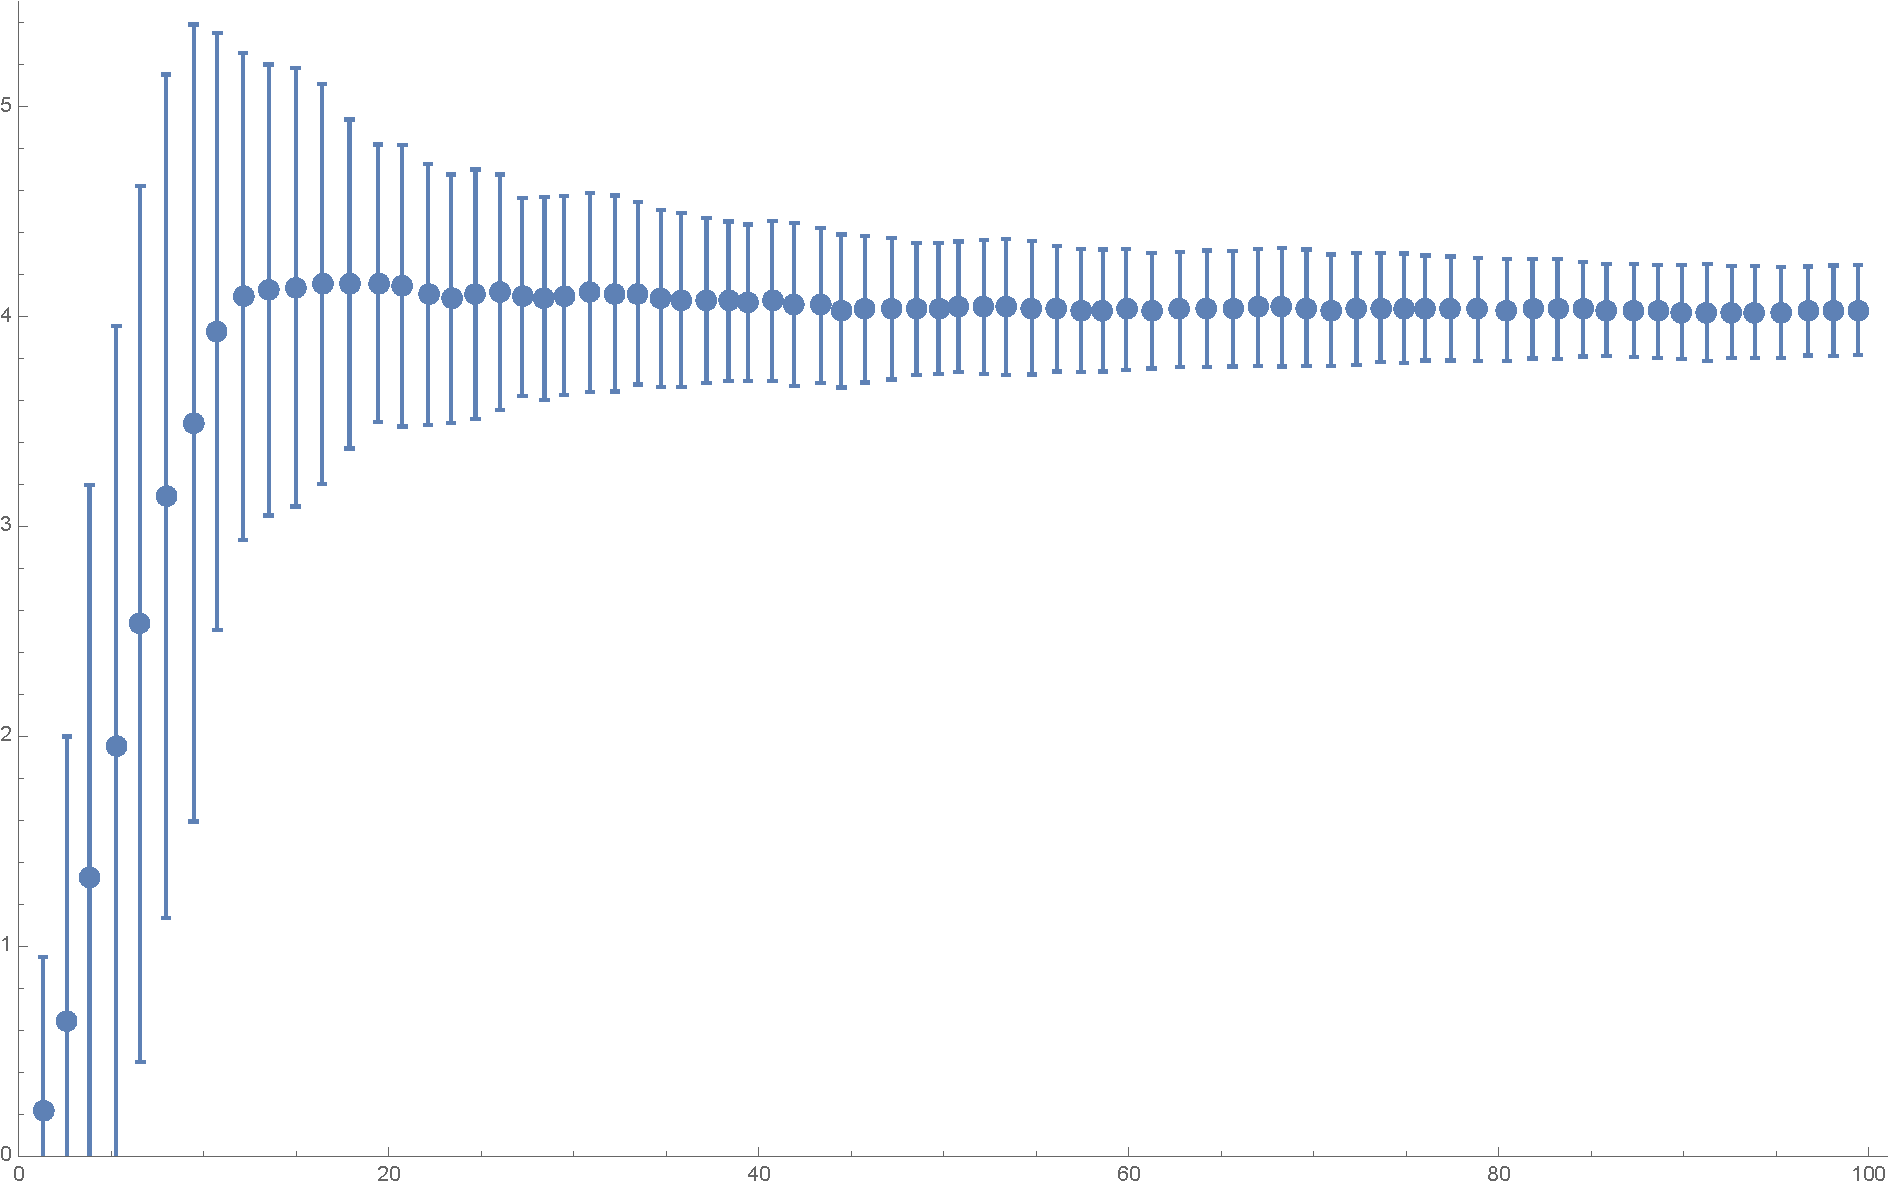
\includegraphics[height=2.5in]{CSDimRedLrg.pdf}
\caption{Myrheim-Meyer dimension for subsets of a relatively large causal set \label{fig1}}
\end{center}
\end{figure}

To investigate the dependence of dimension on volume, one must choose a way to
of select causal sets of ``small" volume.  Since the volume of a causal set is
determined by the number of points in the set, it is tempting to simply average
over all subsets containing a given number of points.  This can be misleading, though:
while such sets are ``small" if viewed outside the context of the background
spacetime, most of them do not come from a small region of the background spacetime,
but include points spread across a large region of the background manifold.   In
particular, two points with a lightlike separation can be ``adjacent'' in a causal set
even if they are widely separated in spacetime.

As an alternative, for each of our sprinklings we considered successively smaller sub-diamonds
in the background spacetime.  The points in each sub-diamond constitute a new causal
set, whose volume and Myrheim-Meyer dimension we computed.  We repeated the
process for 10,000 sprinklings, and then averaged the dimension at
each volume.  We initially applied this analysis to four-dimensional Minkowski space,
but subsequently repeated it for $d=3$ and $d=5$.

As noted above, the Myrheim-Meyer dimension is not well-defined for single points or
causal sets with no edges.  While this concern is unimportant for large causal sets, it
must be confronted for the very small sets  we are interested in.  We explored
two reasonable possibilities: taking the volume of an isolated point to be zero (they are,
after all, single points) or dropping edgeless causal sets from our counting (they
are causally disconnected from the rest of spacetime).

\section{Results}

In each of the background dimensions we studied, we found that dimensional reduction
does indeed occur as the volume decreases.   As shown in figures \ref{fig2}--\ref{fig4},
the process appears to be smooth, but has a rather abrupt onset.  The
transition to lower dimension starts at a volume of approximately $V=8$ points in
three dimensions, $V=16$ points in four dimensions, and $V=22$ points in five
dimensions.\footnote{Fractional volumes appear in the graphs because at a given
background volume in Minkowski space, causal sets with varying numbers of points
may be present.}

At volumes above the transition, the Myrheim-Meyer dimension remains stable and
equal to the dimension of the background Minkowski space.  Below the transition,
the decrease is quite rapid.  For each of the background dimensions we considered,
the minimum Myrheim-Meyer dimension falls to $d_M\approx 0$ if edgeless causal
sets are taken to have dimension zero, and $d_M\approx 2$ if they are omitted.
We can understand the latter result by noting that the smallest causal set with an
edge---two points with one relation---has a Myrheim-Meyer dimension of two.

Figures \ref{fig2}--\ref{fig4} show $1\, \sigma$ error bars.  We believe these are not
a result of poor statistics, but are rather a consequence of our definition of
volume.  A causal diamond of a given volume in a background Minkowski space can
contain many different causal sets, which will not all have identical Myrheim-Meyer
dimensions.  This leads to a genuine statistical fluctuation in dimension, especially
at small volumes.

The end point $d_M\approx 2$ is reminiscent of the behavior seen in other
investigations of quantum gravity.  More precisely, when edgeless causal
sets are discarded, we find a minimum dimension of $d_M = 2.08 \pm .26$ in three
background dimensions, $d_M = 2.13 \pm .39$ in four background dimensions, and
$d_M = 2.19 \pm .40$ in five background  dimensions.  It would be interesting to
understand the fluctuations better, especially since a few other approaches to
quantum gravity suggest a minimum dimension of $3/2$

We would also like to understand what determines the scale at which dimensional
reduction sets in.  For three and four background dimensions, the transition seems to
occur at a characteristic length of about twice the sprinkling length---that is,
$V\sim 2^d$ points---but this pattern appears to break down for background
 dimension five.  We also plan to investigate the behavior of another standard
dimensional estimator, midpoint scaling dimension 

Ideally, we would like to do more.  The results we have presented here have the
awkward feature of relying on the background Minkowski space to define the
small regions whose dimension we measure.  This was necessary to avoid picking
out causal subsets that were ``small'' in the sense of having few points, but
``large'' in the sense of occupying a highly extended region.  Recently, some
progress has been made in defining ``local'' regions entirely in the context of
causal sets, without reference to any background .  It might be
possible to use this work to investigate dimensional reduction more intrinsically.



\begin{figure}
\begin{center}
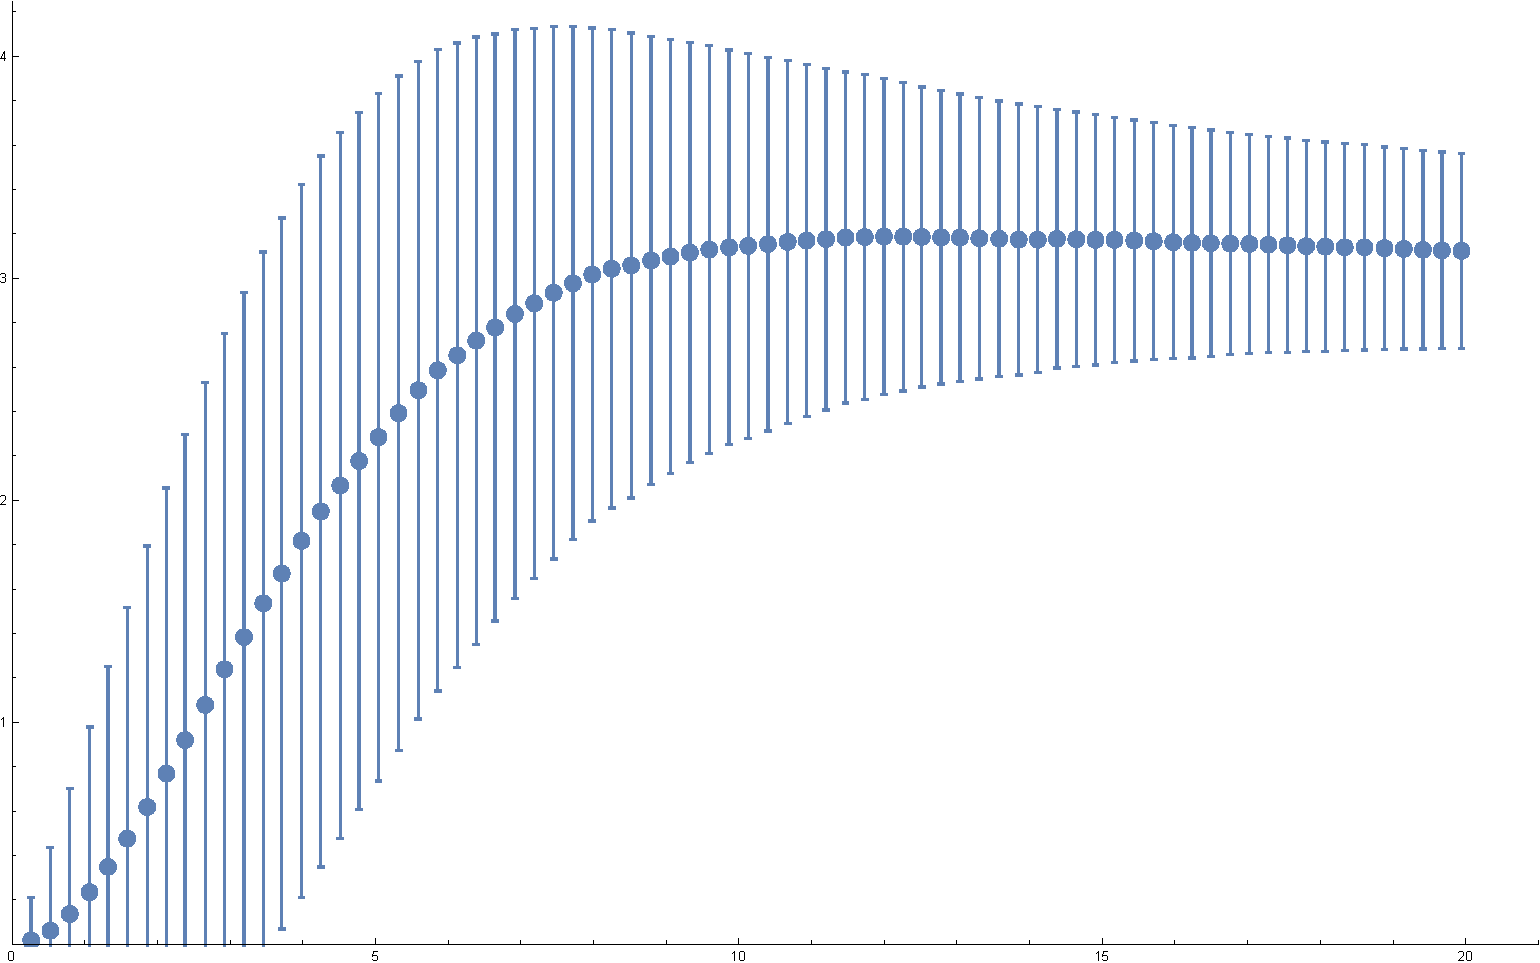
\includegraphics[width=3.15in]{CSDimRed3D.pdf}
 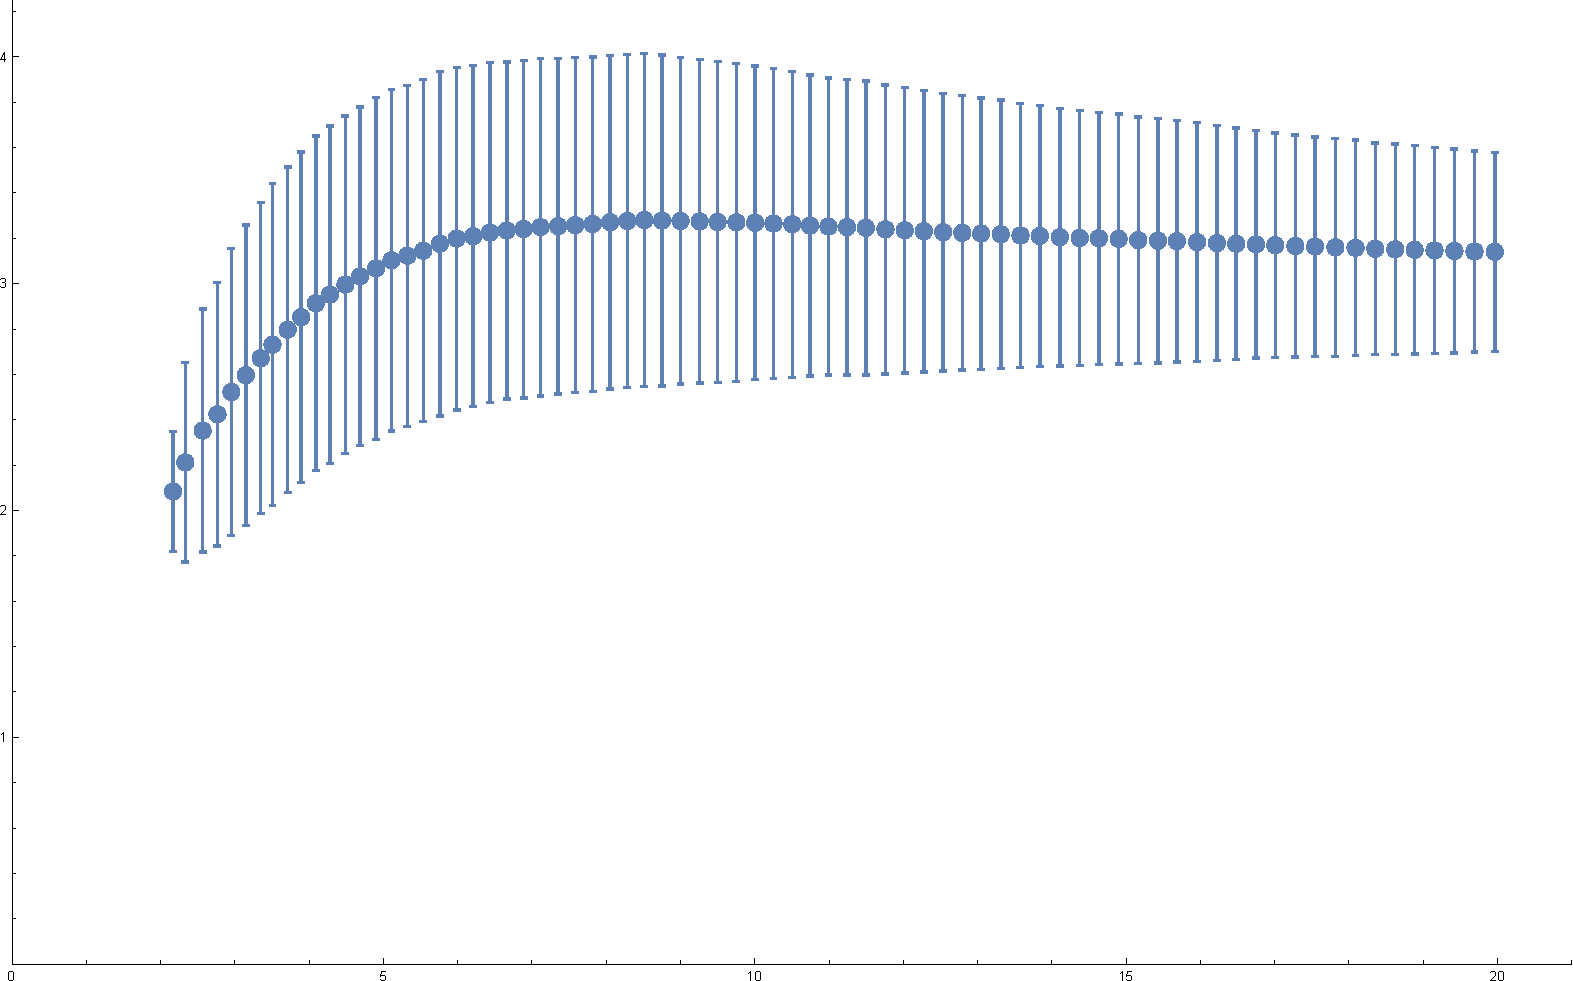
\includegraphics[width=3.15in]{CSDimRed3D2.pdf}
\caption{Myrheim-Meyer dimension in a three-dimensional background,
with edgeless sets counted as dimension zero (left) or omitted (right) \label{fig2}}
\end{center}
\begin{center}
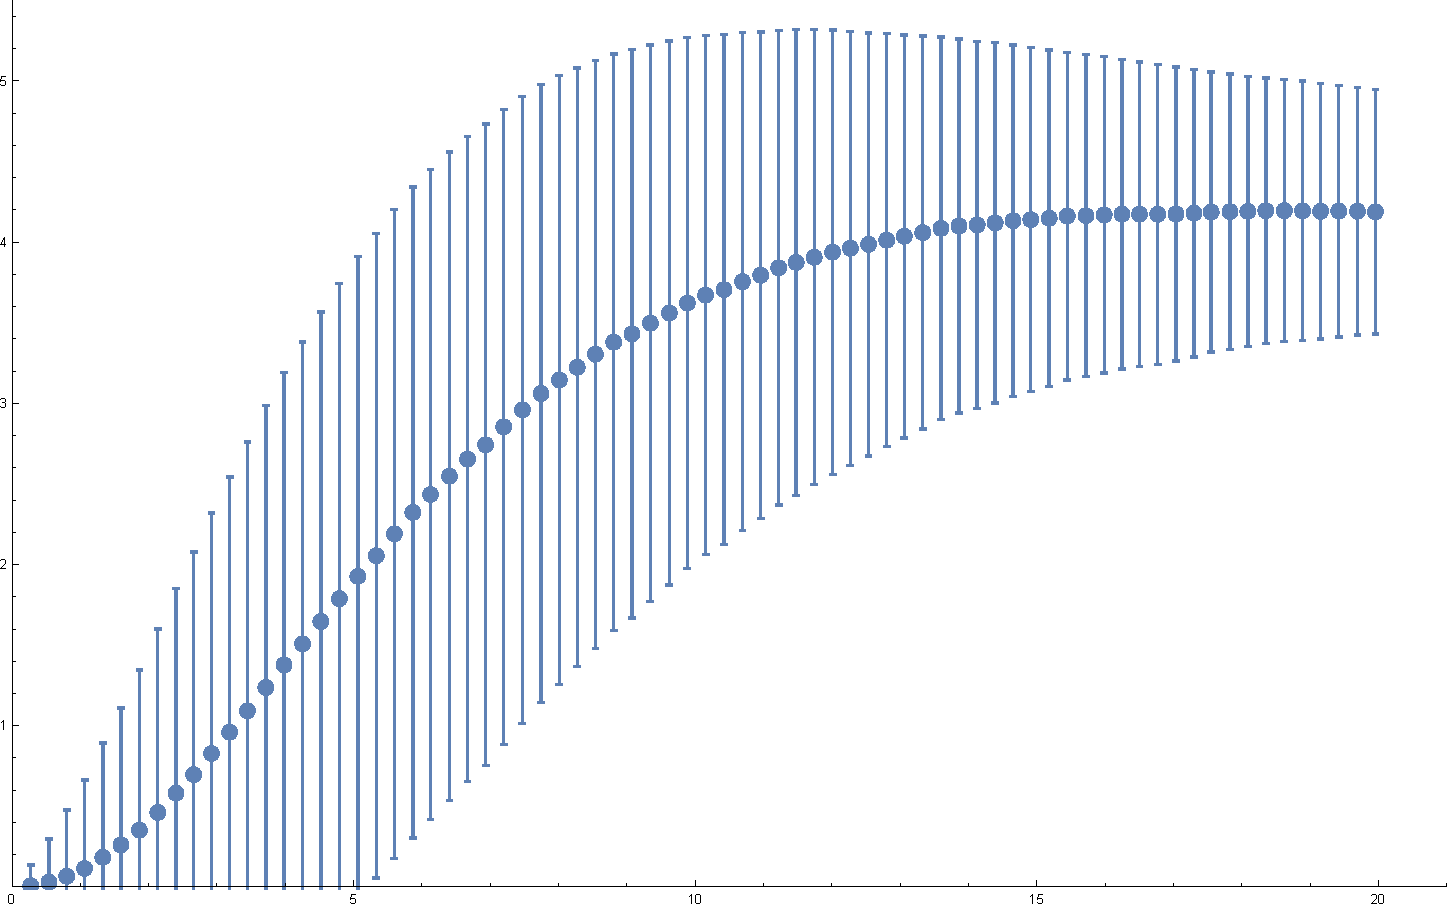
\includegraphics[width=3.15in]{CSDimRed.pdf}
 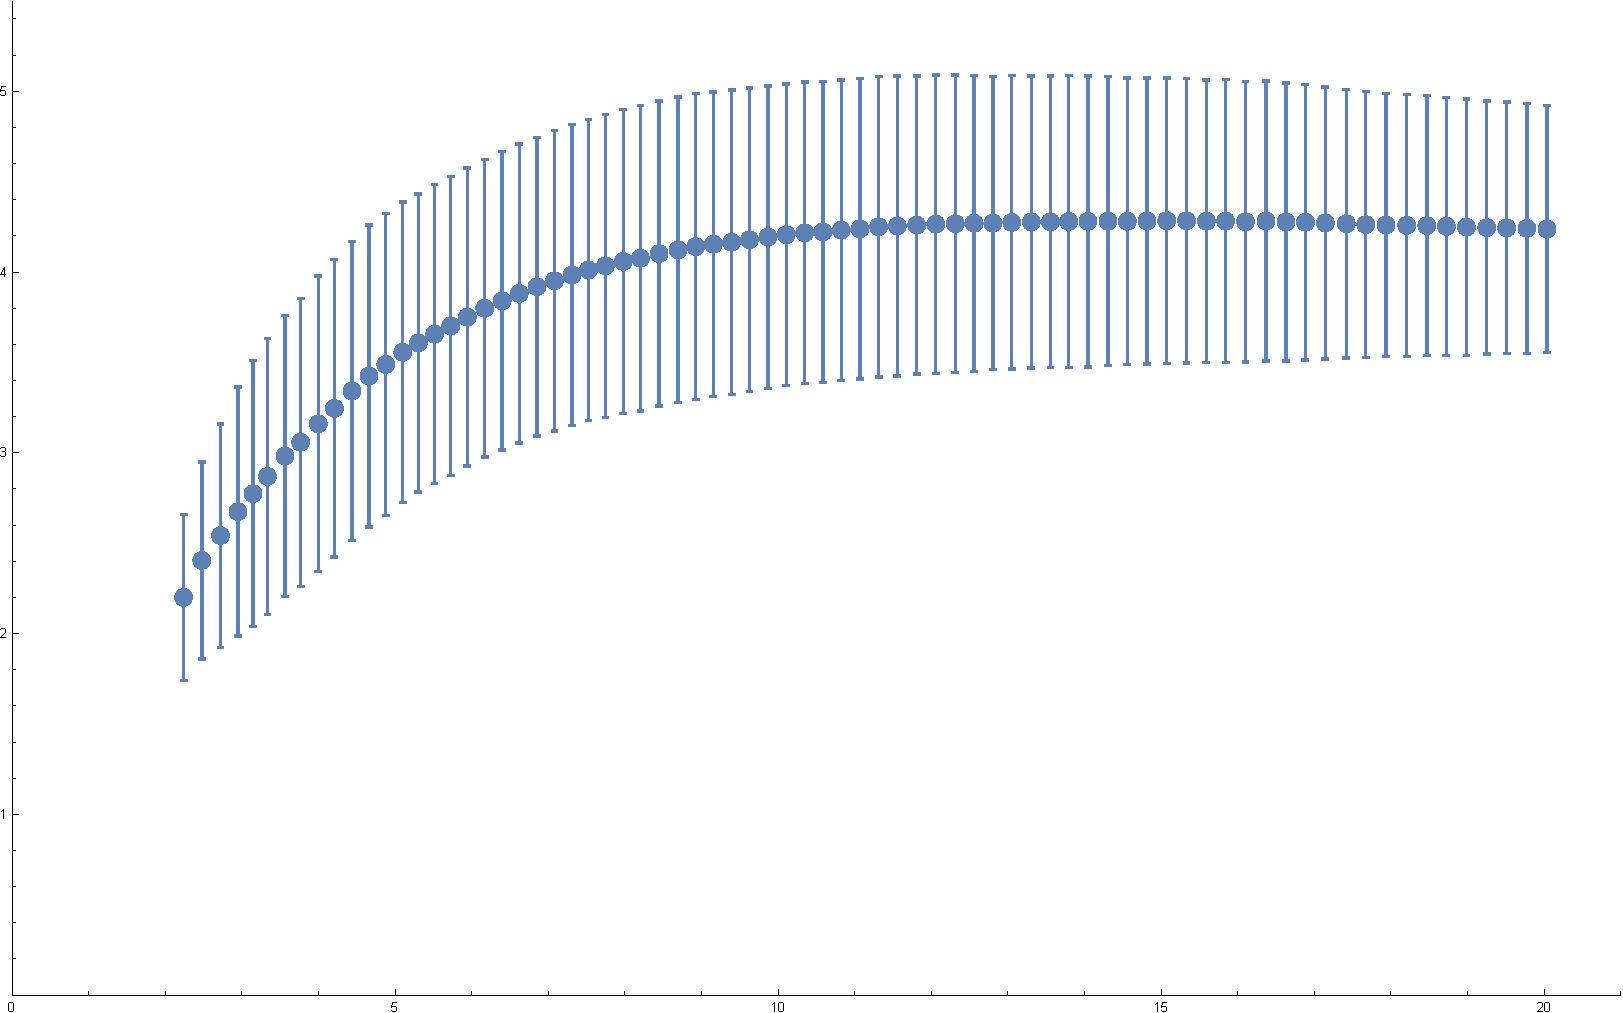
\includegraphics[width=3.15in]{CSDimRed2.pdf}
\caption{Myrheim-Meyer dimension in a four-dimensional background,
with edgeless sets counted as dimension zero (left) or omitted (right) \label{fig3}}
\end{center}
\begin{center}
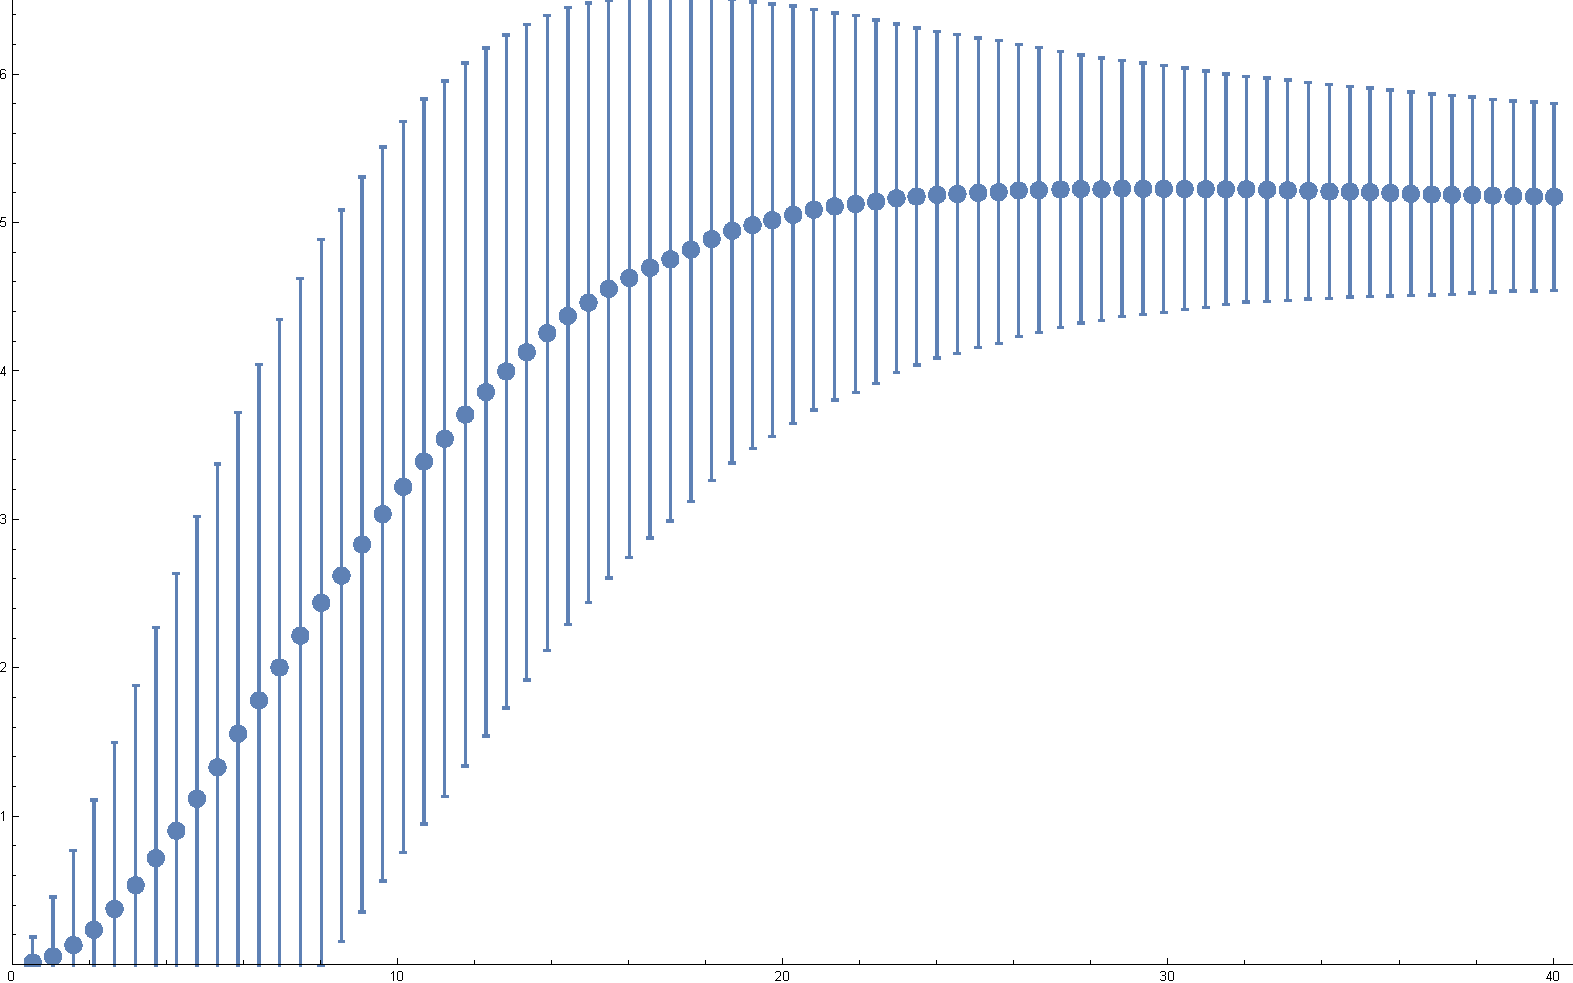
\includegraphics[width=3.15in]{CSDimRed5D.pdf}
 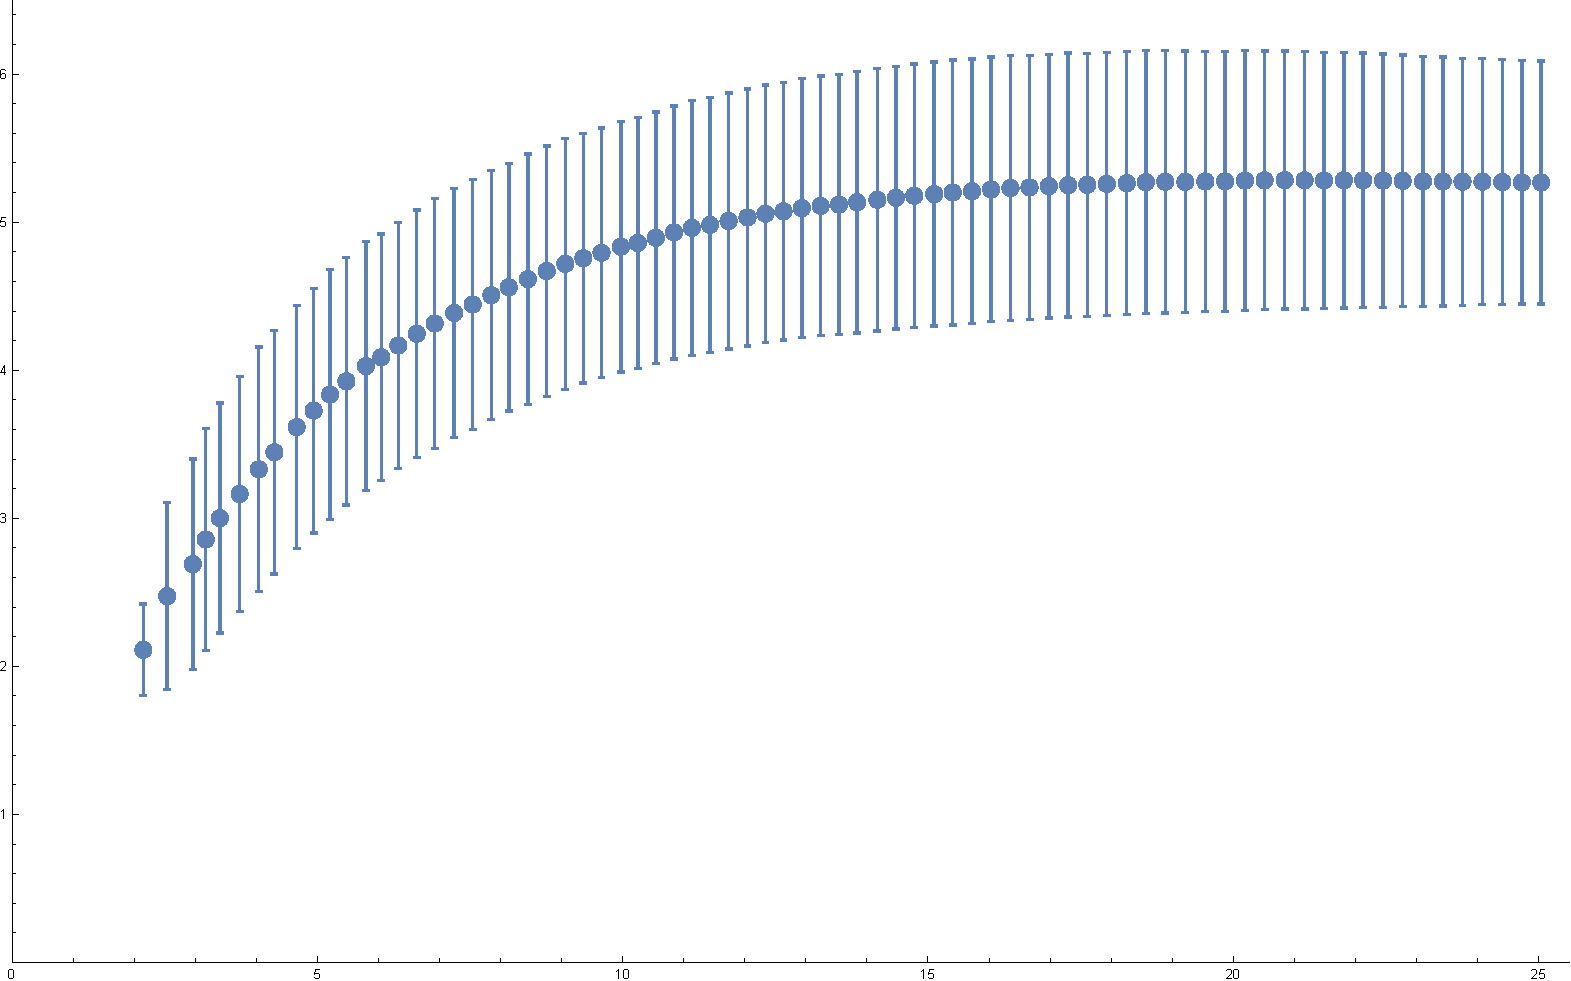
\includegraphics[width=3.15in]{CSDimRed5D2.pdf}
\caption{Myrheim-Meyer dimension in a five-dimensional background,
with edgeless sets counted as dimension zero (left) or omitted (right) \label{fig4}}
\end{center}
\end{figure}

\newpage

\vspace{1.5ex}

\bibliographystyle{ieeetr}
\bibliography{EfficientCDT.bib}
\end{document}
